\documentclass[10pt,a4paper]{article}
\usepackage[a4paper, top=2cm, bottom=1.5cm, left=1.5cm, right=1.5cm]{geometry} % Задать размеры полей.
\usepackage[warn]{mathtext} % Русские символы в формулах. Нужно писать до пакета babel. Указывает, что в формулах используются символы кириллицы, которые по умолчанию печатаются прямым шрифтом.
\usepackage[T2A]{fontenc}
\usepackage[utf8]{inputenc}
\usepackage[russian]{babel}
\usepackage{amsmath}
\usepackage{amssymb}
\usepackage{graphicx}

\usepackage{caption} % Для заголовков таблиц
\DeclareCaptionLabelSeparator{colon}{ }
\DeclareCaptionLabelFormat{table-fmt}{\textbf{#1 #2.}}
\captionsetup[table]{labelformat=table-fmt,skip=0pt,singlelinecheck=off}

\usepackage{booktabs}
\usepackage{wrapfig}
\usepackage{fancyhdr}
\usepackage{multicol}
\usepackage{xcolor}

\usepackage{float}
\usepackage{multirow}

\usepackage{subfigure}

% Объявляем новую команду для переноса строки внутри ячейки таблицы
\newcommand{\specialcell}[2][c]{%
	\begin{tabular}[#1]{@{}c@{}}#2\end{tabular}}

\newcommand{\figref}[1]{(См. рис. \ref{#1})}
\newcommand{\secref}[1]{(См. раздел. \ref{#1})}

\newcommand{\angstrom}{\text{\normalfont\AA}}
\newcommand{\e}[1]{\text{$\cdot10^{#1}$}}
\newcommand{\m}{\; м}
\newcommand{\mm}{\; мм}
\newcommand{\um}{\; мкм}
\newcommand{\A}{\; А}
\newcommand{\V}{\; В}
\newcommand{\uV}{\; мкВ}
\newcommand{\cels}{\; ^\circ С}

\pagestyle{fancy}
\fancyhead{}
\fancyhead[L]{\small Дедков Д.А., Маслов А.С., Изучение рассеяния медленных электронов на атомах. Эффект Рамзауэра. МФТИ, 2023 г.}
\fancyhead[R]{}
\fancyfoot[C]{\thepage}

\renewcommand{\cot}{\text{ctg}}

\author{\normalsize Дедков Денис, Маслов Артём \\
	\normalsize группа Б01-108а \\
	\normalsize 27.11.2023}
\date{}

\title{
	\Large Изучение рассеяния медленных электронов на атомах. Эффект Рамзауэра. \\ 
}

\begin{document}
\maketitle
	
	\subsection*{Цель и задачи работы:}
	\begin{enumerate}
		\item Исследовать энергетические зависимости вероятности рассеяния электронов атомами инертного газа. 
		
		\item Определить энергии электронов, при которых наблюдается просветление инертного газа.
		
		\item Оценить размер внешней электронной оболочки инертного газа.
		
		\item По значению измеренного ионизационного потенциала определяется, каким газом заполнен тиратрон.
	\end{enumerate}
	
	\subsection*{Описание экспериментальной установки}
	
	\begin{figure}[H]
		\centering
		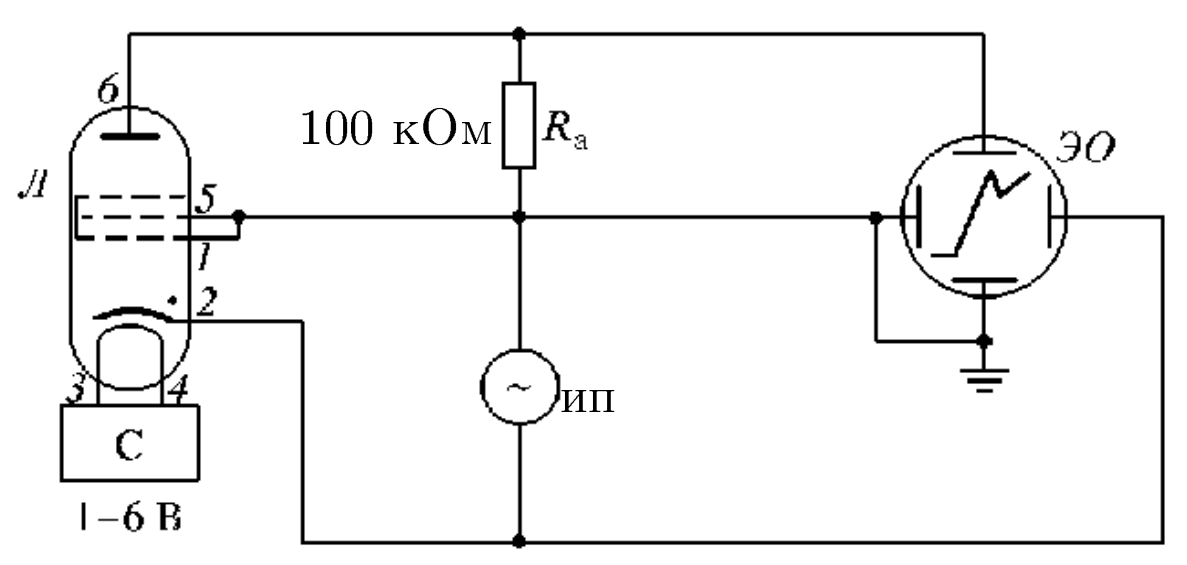
\includegraphics[width=0.3\textwidth]{img/schm1.png}
		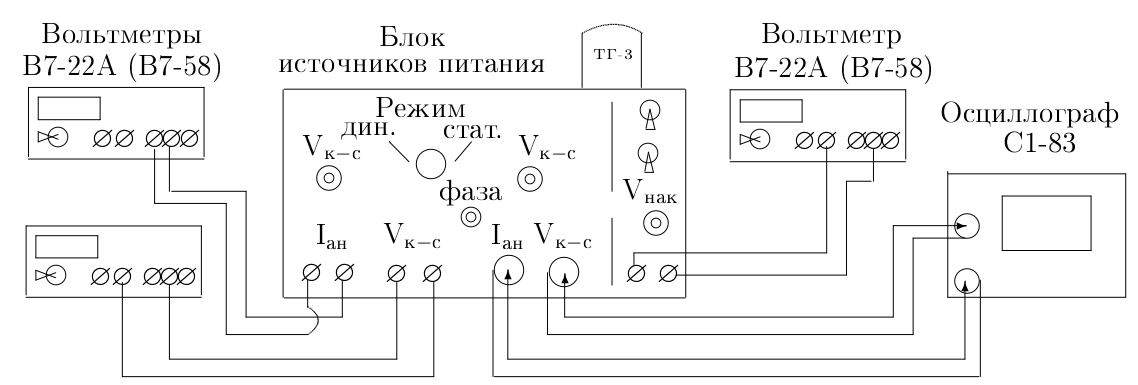
\includegraphics[width=0.6\textwidth]{img/schm2.png}
		\caption{Слева схема подключения тиратрона. Справа блок-схема экспериментальной установки.}
		\label{img:exp_scheme}
	\end{figure}

	\begin{wrapfigure}{r}{0.3\textwidth}
		\centering
		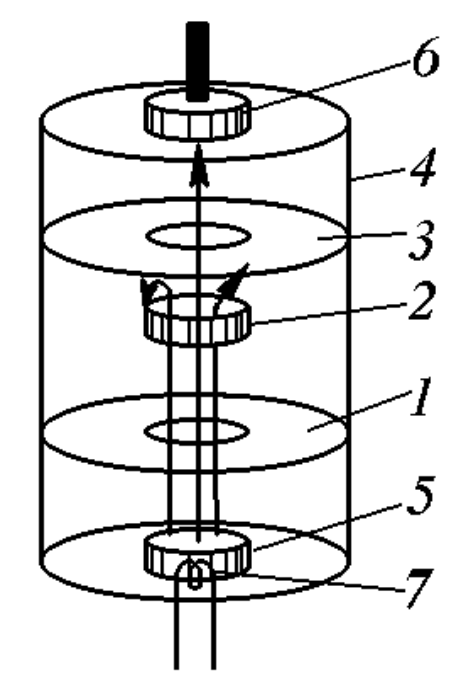
\includegraphics[width=0.15\textwidth]{img/tiratron.png}
		\caption{Схема тиратрона: 1, 2, 3 -- сетки с одинаковым потенциалом, 4 -- внешний металлический цилиндр, 5 -- катод, 6 -- анод, 7 -- накаливаемая спираль.}
		\label{img:tiratron}
	\end{wrapfigure}

	В работе для наблюдения эффекта Рамзауэра используется тиратрон ТГ3-01/1.3Б, заполненный инертным газом (рис. \ref{img:tiratron}). Электроны, эмитируемые катодом тиратрона, ускоряются напряжением $V$, приложенным между катодом и ближайшей к нему сеткой. Затем электроны рассеиваются на атомах инертного газа. Рассеянные электроны отклоняются в сторону и уходят на сетку, а оставшаяся часть электронов достигает анода и создаёт анодный ток $I_а$.
	
	Схема экспериментальной установки приведена на рисунке \ref{img:exp_scheme}. Лампа тиратрона расположена на корпусе блок источников питания. Напряжение к электродам лампы подаётся от источников питания, находящихся в корпусе прибора. Регулировка напряжения и выбор режима работы установки производится при помощи ручек управления, выведенных на лицевую панель блока источников питания.	
	
	\subsection*{Оборудование и приборы}
		
	Стенд с экспериментальной установкой номер $1.3._1$.
	\begin{enumerate}
		\item Тиратрон ТГ3-01/1.3Б.
				
		\item Вольтметры GDM-8145. Инвентарный номер вольтметра, измеряющего напряжение, пропорциональное току анода, №210104003098. Инвентарный номер вольтметра, измеряющего напряжение катод-сетка, №210104003102. Инвентарный номер вольтметра, измеряющего напряжение накала тиратрона, №210104003100. Все вольтметры измеряют в пределе 20 В. Погрешность измерения $\sigma = \pm (0.03\% \; rdg + 4 \; digits)$.
		
		\item Блок источников питания. Заводской номер №606-502. Инвентарный номер №410134125767.
		
		\item Осциллограф GOS-620. Инвентарный номер №210104000620. Коэффициент отклонения $4\%$ в диапазоне $5 \; \frac{мВ}{дел} \div 5 \; \frac{В}{дел}$.
	\end{enumerate}
	
	\subsection*{Первичные экспериментальные данные}
	
	Первичные экспериментальные данные приведены в таблицах \ref{table:first}-\ref{table:last}.
	
	\begin{table}[H]
		\caption[table]{Статический режим. $V_{накала} = 2.52 \V$.}
		\label{table:first}
		\begin{center}
			\input{gen/tab-2.52V.tex}
		\end{center}
		\caption*{$V_{катод}$ -- напряжение катод-сетка, $V_{анод}$ -- напряжение анод-сетка. Погрешность измерения напряжения определяется погрешностью измерения вольтметра $\sigma_{приб} = \pm (0.03\% \; rdg + 4 \; digits)$; шумом в электрической схеме, погрешность шума оцениваем как среднеквадратичное отклонение нескольких измерений $\sigma_{шум}^{катод} = 0.01 \V$, $\sigma_{шум}^{анод} = 0.1 \; мВ$. Ток анода вычислялся по формуле $I_{анод} = R V_{анод}$, погрешность оценивается как $\sigma_{I_{анод}} = I_{анод} \cdot \sqrt{\varepsilon_R^2 + \varepsilon_{V_{анод}}^2}$, где $\varepsilon_R = 10 \%$ -- допустимое отклонение сопротивления резистора от номинального.}
	\end{table}

	\begin{table}[H]
		\caption{Статический режим. $V_{накала} = 2.75 \V$.}
		\begin{center}
			\input{gen/tab-2.75V.tex}
		\end{center}
		\caption*{$V_{катод}$ -- напряжение катод-сетка, $V_{анод}$ -- напряжение анод-сетка. Погрешность измерения напряжения определяется погрешностью измерения вольтметра $\sigma_{приб} = \pm (0.03\% \; rdg + 4 \; digits)$; шумом в электрической схеме, погрешность шума оцениваем как среднеквадратичное отклонение нескольких измерений $\sigma_{шум}^{катод} = 0.01 \V$, $\sigma_{шум}^{анод} = 0.1 \; мВ$. Ток анода вычислялся по формуле $I_{анод} = R V_{анод}$, погрешность оценивается как $\sigma_{I_{анод}} = I_{анод} \cdot \sqrt{\varepsilon_R^2 + \varepsilon_{V_{анод}}^2}$, где $\varepsilon_R = 10 \%$ -- допустимое отклонение сопротивления резистора от номинального.}
	\end{table}
	
	\begin{table}[H]
		\caption{Динамический режим.}
		\label{table:last}
		\begin{center}
			\input{gen/tab-dyn.tex}
		\end{center}
		\caption*{$V_{накал}$ -- напряжение накала тиратрона, погрешность измерения одинакова и определяется точностью вольтметра и шумами в электрической цепи $\sigma_{V_{накал}} = 0.01 \V$. $V_{мин}$ -- напряжение минимума, $V_{макс}$ -- напряжение максимума, $V_{break}$ -- напряжение пробоя. Погрешность $V_{мин}$, $V_{макс}$ и $V_{break}$ определяется погрешность измерения напряжения по осциллографу $\varepsilon_{осц} = 4\%$ и ошибкой, связанной с определением положения максимума. Погрешность определения максимума связана с шириной линии на экране осциллографа. Данные с осциллографа оцифровывались для увеличения точности измерения и удобства обработки измеренных данных: делалась фотография измеряемого сигнала так чтобы плоскость камеры была параллельная плоскости экрана осциллографа и изображение было четким (камера сфокусирована на экране осциллографа), затем координаты максимумов измерялись в пикселях на компьютере и переводились в соответствие со шкалой прибора, отградуированной в пикселях. При этом возникает дополнительная погрешность, связанная с конечным разрешением камеры. Погрешность определения положения максимума сигнала оценим как ширину наблюдаемой на экране осциллографа линии, которая была настроена максимально тонкой и яркой при измерениях. Ширина линии сигнала составляет $~12$ пикселей, погрешность, связанная с конечным разрешением камеры составляет $\sim 1$ пиксель. Тогда погрешность снятия показаний с осциллографа  $\sigma_{цифр} = \sqrt{12^2 + 1^2} \approx 12$ пикселей, что соответствует $\sigma_{цифр} = 0.3 \V$. Общая погрешность $\sigma_{осц} = \sqrt{\sigma_{цифр}^2 + (V_{измер} \cdot \varepsilon_{осц})^2}$. Также существует ошибка определения напряжения, связанная с наличием контактной разности потенциалов, оценить которую напрямую не удаётся.}
	\end{table}
	
	\subsection*{Обработка экспериментальных данных}
	
	\subsubsection*{Динамический режим}
	
	По результатам измерения в динамическом режиме определим эффективный размер (диаметр) электронной оболочки атома инертного газа
	$$
	l = \frac{h\sqrt{5}}{\sqrt{32 m_e e (V_{мин} - V_{макс})}}
	$$
	и эффективную глубину потенциальной ямы атома
	$$
	U_0 = e \left(\frac{4}{5} V_{мин} - \frac{9}{5} V_{макс} \right)
	$$
	Оценим погрешность $l$ по формуле косвенных измерений:
	$$
	\sigma_l = \frac{1}{2} l \cdot \frac{\sqrt{\sigma_{V_{мин}}^2 + \sigma_{V_{макс}}^2}}{V_{мин} - V_{макс}}
	$$
	Оценим погрешность $U_0$ по формуле косвенных измерений:
	$$
	\sigma_{U_0} = \sqrt{\left(\frac{4}{5} \sigma_{V_{мин}}\right)^2 + \left(\frac{9}{5} \sigma_{V_{макс}}\right)^2}
	$$
	
	При измерении напряжение осциллографом существует ошибка, связанная с наличием контактной разности потенциалов, оценить которую напрямую не удаётся. С другой стороны, при вычислении эффективного размера электронной оболочки атома $l$ используются значения напряжение не по отдельности, а их разность. В предположении, что контактная разность потенциалов не зависит от значения измеряемого напряжения, при вычислении $l$ контактная разность потенциалов не влияет на итоговый результат, тем не менее она вносит дополнительную ошибку при нахождении эффективной глубины потенциальной ямы атома $U_0$.
	
	Результаты вычислений приведены в таблице \ref{table:atom}.
	
	\begin{table}[H]
		\caption{Динамический режим. Эффективный размер электронной оболочки атома $l$ и эффективная глубина потенциальной ямы атома $U_0$.}
		\label{table:atom}
		\begin{center}
			\input{gen/tab-dyn-atom.tex}
		\end{center}
	\end{table}

	Геометрические размеры тиратрона таковы, что ионизационный потенциал практически совпадает с напряжением пробоя. Среднее значение напряжения пробоя: \\
	$$
	U_{пробой} = 12 \pm 1 \V
	$$
	Погрешность определяется по формуле
	$$
	\sigma_{U_{пробой}} = \sqrt{\sigma_{приб}^2 + \sigma_{случ}^2} = 1.1 \V
	$$
	$$
	\sigma_{случ} = \sqrt{\frac{1}{N - 2}\sum_i \frac{\left(U_i - \overline{U}\right)^2}{N}} = 0.9 \V
	$$
	Приборную погрешность измерения среднего напряжения оценим как среднюю погрешность отдельных измерений $\sigma_{приб} = 0.6 \V$.
	Итого, ионизационный потенциал
	$$
	U_{ион} = 12 \pm 1 \; эВ
	$$
	что совпадает с ионизационным потенциалом ксенона $U_{ион}^{Xe} = 12.1 \; эВ$.
	
	\subsubsection*{Статический режим}

	Построим графики зависимости $I_{анод}(V_{катод})$ при разных напряжениях накала тиратрона.

	\begin{figure}[H]
		\centering
		\includegraphics[width=0.7\textwidth]{gen/static.pdf}
		\caption{График зависимости тока анода $I_{анод}$ от напряжения катода $V_{катод}$.}
	\end{figure}
	
	По графику $I_{анод}(V_{катод})$ определим напряжения максимумов и минимумов.
	
	\begin{table}[H]
		\caption{Статический режим. Напряжения максимумов и минимумов на графике $I_{анод}(V_{катод})$}
		\label{table:st}
		\begin{center}
			\input{gen/tab-st.tex}
		\end{center}
		\caption*{$V_{накал}$ -- напряжение накала тиратрона, погрешность измерения одинакова и определяется точностью вольтметра и шумами в электрической цепи $\sigma_{V_{накал}} = 0.01 \V$. $V_{мин}$ -- напряжение минимума, $V_{макс}$ -- напряжение максимума.}
	\end{table}

	Определим эффективный размер электронной оболочки атома $l$ и эффективная глубина потенциальной ямы атома $U_0$.
	
	\begin{table}[H]
		\caption{Статический режим. Эффективный размер электронной оболочки атома $l$ и эффективная глубина потенциальной ямы атома $U_0$.}
		\label{table:atom-st}
		\begin{center}
			\input{gen/tab-st-atom.tex}
		\end{center}
	\end{table}

	Построим график зависимости вероятности рассеяния электронов (с точностью до константы) от энергии:
	$$
	w(V) = -\frac{1}{C} \ln{\frac{I_{анод}(V)}{I_0}}
	$$
	\begin{figure}[H]
		\centering
		\includegraphics[width=0.7\textwidth]{gen/probability.pdf}
		\caption{График зависимости вероятности в условных единицах от напряжения катод-сетка $V_{катод}$.}
	\end{figure}

	\subsection*{Обсуждение результатов и выводы}
	
	В работе были оценены эффективные размеры электронной оболочки атома инертного газа и эффективная глубина потенциальной ямы статическим и динамическим методами.
	\begin{table}[H]
		\caption*{Динамический режим. Эффективный размер электронной оболочки атома $l$ и эффективная глубина потенциальной ямы атома $U_0$.}
		\begin{center}
			\input{gen/tab-dyn-atom.tex}
		\end{center}
	\end{table}
	
	\begin{table}[H]
		\caption*{Статический режим. Эффективный размер электронной оболочки атома $l$ и эффективная глубина потенциальной ямы атома $U_0$.}
		\begin{center}
			\input{gen/tab-st-atom.tex}
		\end{center}
	\end{table}
	
	\begin{table}[H]
		\caption*{Значения эффективных размеров электронных оболочек атомов из справочника: E. Clementi; D.L.Raimondi; W.P. Reinhardt (1967). "Atomic Screening Constants from SCF Functions. II. Atoms with 37 to 86 Electrons". The Journal of Chemical Physics. 47 (4): 1300–1307.}
		\begin{center}
			\begin{tabular}{ccc}
				\hline
				& $l_e, \angstrom$ & $l_c, \angstrom$ \\
				\hline
				$Ar$ & 1.42 & 1.42 \\
				$Kr$ & --- & 1.76 \\
				$Xe$ & --- & 2.16 \\
				\hline
			\end{tabular}
		\end{center}
		\caption*{$l_e$ -- диаметр внешней электронной оболочки, полученный на основе экспериментальных данных. Если указан прочерк, то таких данных нету. $l_c$ -- диаметр внешней электронной оболочки, полученный на основе теоретических моделей.}
	\end{table}
	
	С помощью динамического метода был определён ионизационный потенциал инертного газа:
	$$
	U_{ион} = 12 \pm 1 \; эВ
	$$
	что совпадает с ионизационным потенциалом ксенона $U_{ион}^{Xe} = 12.1 \; эВ$. Поэтому можно предположить, что в тиратроне находится ксенон.
	
\end{document}